\documentclass{article}

\usepackage[utf8]{inputenc}
\usepackage[T1]{fontenc}
\usepackage{lmodern}
\usepackage[polish]{babel}
\usepackage[margin=1in]{geometry}

\usepackage{amsmath}
\usepackage{amsfonts}
\usepackage{amssymb}

\usepackage{booktabs} % Lepsza jakość tabel
\usepackage{graphicx}
\usepackage{float}

\usepackage{siunitx} 
\sisetup{
    output-exponent-marker = e,
    bracket-numbers = false,
    group-separator = {\,}, 
    scientific-notation = true
}

% Inne
\usepackage{hyperref} 
\hypersetup{
    colorlinks=true,
    linkcolor=blue,
    filecolor=magenta,      
    urlcolor=cyan,
    pdftitle={Obliczenia Naukowe - Lista 1},
    pdfauthor={Wojciech Typer},
}

\title{Sprawozdanie z Laboratorium\\Obliczenia Naukowe - Lista 1}
\author{Wojciech Typer}

\begin{document}
\maketitle
\section*{Zadanie 1}

\subsection{Epsilon maszynowy (\textit{macheps})}

Epsilonem maszynowym \textit{macheps} nazywamy najmniejszą liczbę dodatnią taką, że w arytmetyce zmiennoprzecinkowej zachodzi \(1.0 + \text{macheps} > 1.0\). Jest to miara precyzji obliczeń, która określa odległość od liczby 1.0 do następnej reprezentowalnej liczby maszynowej. Im mniejszy epsilon, tym większa precyzja arytmetyki, co jest bezpośrednio związane z liczbą bitów przeznaczonych na mantysę w danym typie zmiennoprzecinkowym.

Poniżej przedstawiono porównanie wartości \textit{macheps} uzyskanych iteracyjnie, wartości zwracanych przez funkcję \texttt{eps()} w Julii oraz wartości zdefiniowanych w pliku nagłówkowym \texttt{float.h} kompilatora C (GCC 13).

\begin{table}[H]
\centering
\caption{Porównanie wartości epsilona maszynowego.}
\label{tab:epsilon}
\begin{tabular}{llll}
\toprule
\textbf{Typ danych} & \textbf{Wartość z \texttt{float.h} (GCC)} & \textbf{Wartość z \texttt{eps(T)} (Julia)} & \textbf{Wartość wyznaczona iteracyjnie} \\
\midrule
\texttt{Float16} & \num{9.7656e-4} & \num{0.000977} & \num{0.000977} \\
\texttt{Float32} & \num{1.192093e-07} & \num{1.1920929e-7} & \num{1.1920929e-7} \\
\texttt{Float64} & \num{2.220446e-16} & \num{2.220446049250313e-16} & \num{2.220446049250313e-16} \\
\bottomrule
\end{tabular}
\end{table}

Jak widać w tabeli \ref{tab:epsilon}, wartości uzyskane eksperymentalnie są zgodne z wartościami referencyjnymi. 

\textbf{Związek między macheps a $\epsilon$}: Porównując wartość macheps z wartościami precyzji arytmetyki podanymi na wykładzie,
to możemy zauważyć następującą zależność: $\text{macheps} = 2 \cdot \epsilon$. %Oznacza to, że epsilon maszynowy jest dwukrotnością wartości $\epsilon$ definiowanej jako odległość między 1.0 a następną reprezentowalną liczbą maszynową.

\subsection{Najmniejsza dodatnia liczba maszynowa (\textit{eta})}

Liczba \textit{eta} (\(\eta\)) to najmniejsza dodatnia wartość, jaką można reprezentować w danym standardzie zmiennoprzecinkowym. Wartość ta jest związana z liczbami subnormalnymi (denormalizowanymi), które pozwalają na płynne "wypełnienie" luki między zerem a najmniejszą dodatnią liczbą znormalizowaną.

\begin{itemize}
    \item \textbf{Związek z \textit{MIN\textsubscript{sub}}}: Liczba \textit{eta} jest tożsama z \textit{MIN\textsubscript{sub}}, czyli najmniejszą możliwą do reprezentowania dodatnią liczbą subnormalną. W języku Julia wartość tę można uzyskać za pomocą funkcji \texttt{nextfloat(T(0.0))}.
    \item \textbf{Związek z \textit{MIN\textsubscript{nor}}}: Funkcja \texttt{floatmin(T)} zwraca najmniejszą dodatnią liczbę \textbf{znormalizowaną}, znaną jako \textit{MIN\textsubscript{nor}}. Dla odpowiednio \texttt{Float32} i \texttt{Float64} wartości te wynoszą: \num{1.1754944e-38} i \num{2.2250738585072014e-308}, co zgadza się z wartościami podanymi na wykładzie.
\end{itemize}


Wartości \textit{eta} wyznaczone iteracyjnie (poprzez dzielenie 1.0 przez 2 aż do uzyskania 0.0) są zgodne z wynikami funkcji \texttt{nextfloat(T(0.0))}. Porównanie tych wartości przedstawiono w tabeli \ref{tab:eta}.

\begin{table}[H]
\centering
\caption{Porównanie wartości \textit{eta} (\(\eta\)).}
\label{tab:eta}
\begin{tabular}{lll}
\toprule
\textbf{Typ danych} & \textbf{Wartość z \texttt{nextfloat(T(0.0))}} & \textbf{Wartość wyznaczona iteracyjnie} \\
\midrule
\texttt{Float16} & \num{6.0e-8} & \num{6.0e-8} \\
\texttt{Float32} & \num{1.0e-45} & \num{1.0e-45} \\ 
\texttt{Float64} & \num{5.0e-324} & \num{5.0e-324} \\
\bottomrule
\end{tabular}
\end{table}


\subsection{Największa wartość skończona (\textit{MAX})}

Liczba \textit{MAX} to największa skończona wartość, jaką można zapisać w danym typie zmiennoprzecinkowym. Próba reprezentacji liczby większej niż \textit{MAX} prowadzi do uzyskania wartości nieskończonej (\texttt{Inf}). Doświadczalne wyznaczenie tej wartości polega na iteracyjnym mnożeniu liczby przez 2, aż do momentu, gdy stanie się ona nieskończona, a następnie cofnięciu ostatniej operacji.

\begin{table}[H]
\centering
\caption{Porównanie maksymalnych wartości zmiennoprzecinkowych.}
\label{tab:max}
\begin{tabular}{llll}
\toprule
\textbf{Typ danych} & \textbf{Wartość z \texttt{float.h} (GCC)} & \textbf{Wartość wyznaczona iteracyjnie} & \textbf{Wartość z \texttt{floatmax(T)} (Julia)} \\
\midrule
\texttt{Float16} & --- & \num{6.55e4} & \num{6.55e4} \\
\texttt{Float32} & \num{3.4028234663852886e+38} & \num{3.4028235e38} & \num{3.4028235e38} \\
\texttt{Float64} & \num{1.7976931348623157e+308} & \num{1.7976931348623157e308} & \num{1.7976931348623157e308} \\
\bottomrule
\end{tabular}
\end{table}
Jak widać w tabeli \ref{tab:max}, wartości uzyskane eksperymentalnie są zgodne z wartościami referencyjnymi. 


\section*{Zadanie 2}
W tabeli poniżej znajdują się wartości epsilona maszynowego, obliczone metodą Kahana i te, zwrócone przez funkcję \texttt{eps()} w Julii.
\begin{table}[H]
\centering
\label{tab:kahan_comparison}
\begin{tabular}{lll}
\toprule
\textbf{Typ danych} & \textbf{Wartość z metody Kahana} & \textbf{Wartość z \texttt{eps(T)} (Julia)} \\
\midrule
\texttt{Float16} & \num{-0.000977} & \num{0.000977} \\
\texttt{Float32} & \num{1.1920929e-7} & \num{1.1920929e-7} \\
\texttt{Float64} & \num{-2.220446049250313e-16} & \num{2.220446049250313e-16} \\
\bottomrule


\end{tabular}
\end{table}
\paragraph{Wnioski}
\sloppy 
Z powyższej tabeli widzimy, że aby wyrażenie Kahana poprawnie wyznaczało epsilon maszynowy dla wszystkich typów zmiennopozycyjnych,
należy na wynik nałożyć wartość bezwzględną. Błędy w bicie znaku wynikają z reprezentacji rozwinięcia binarnego ułamka $\frac{4}{3}$.
\fussy % Przywróć domyślne ustawienia

\section*{Zadanie 3}

W zadaniu przeanalizowano rozkład liczb zmiennoprzecinkowych w arytmetyce \texttt{double} w różnych przedziałach. Gęstość rozmieszczenia tych liczb, czyli odległość między dwiema kolejnymi reprezentacjami, zależy od przedziału, w którym się znajdujemy. Sprawdzono to eksperymentalnie dla trzech przypadków.

\begin{itemize}
    \item \textbf{Przedział \([1, 2]\):} W arytmetyce \texttt{double}, liczby zmiennoprzecinkowe są rozmieszczone równomiernie na przedziale \([1, 2]\) z krokiem równym $\delta = 2^{-52}$. Oznacza to, że każda kolejna liczba na tym przedziale różni się od poprzedniej o dokładnie $\delta$. Sprawdzono to eksperymentalnie: 1000-krotnie generując losową liczbę z tego przedziału i wyznaczając kolejną liczbę maszynową za pomocą funkcji \texttt{nextfloat()}, różnica między nimi zawsze była równa $\delta$.

    \item \textbf{Przedział \([0.5, 1]\):} Dla tego przedziału krok wynosi $\delta = 2^{-53}$. Każda liczba może być przedstawiona jako: $x = 1 + k \cdot \delta$, gdzie $k$ jest liczbą całkowitą, a $\delta = 2^{-53}$.

    \item \textbf{Przedział \([2, 4]\):} W tym przypadku krok jest większy i wynosi $\delta = 2^{-51}$. Dla tego przedziału każda liczba może być przedstawiona jako: $x = 2 + k \cdot \delta$, gdzie $\delta = 2^{-51}$.
\end{itemize}

Powyższe eksperymenty potwierdzają, że w arytmetyce zmiennoprzecinkowej liczby są rozmieszczone gęściej bliżej zera i rzadziej w miarę oddalania się od niego. Zjawisko to nie jest przypadkowe, lecz wynika bezpośrednio ze sposobu, w jaki liczby są reprezentowane w formacie IEEE 754.
\section*{Zadanie 4}
\begin{itemize}
    \item Liczba znaleziona eksperymentalnie: 1.7935706239891005 - generujemy losową liczbę z przedziału \([1.0, 2.0]\) i sprawdzamy, czy $ x \cdot \frac{1}{x} \neq 1$. 
    \item Najmniejsza liczba z przedziału \([1.0, 2.0]\), dla której zachodzi \(x \cdot \frac{1}{x} \neq 1\) to 1.000000057228997. Iterujemy od 1.0 w górę, aż do momentu, gdy warunek będzie spełniony.
\end{itemize}

\textbf{Wnioski: } Działania w arytmetyce zmiennopozycyjnej obarczone są błędem, który należy brać pod uwagę nawet podczas podstawowych operacji.

\section*{Zadanie 5}

W zadaniu porównano cztery różne metody obliczania iloczynu skalarnego wektorów, aby zbadać ich stabilność numeryczną i wpływ na błędy zaokrągleń. Wyniki dla precyzji 32-bitowej (\texttt{Float32}) oraz 64-bitowej (\texttt{Float64}) przedstawiono w tabeli \ref{tab:sum_methods}. \\

\begin{table}[H]
\centering
\label{tab:sum_methods}
\begin{tabular}{lllS[table-format=1.18e-1]} % 'S' z siunitx do wyrównania liczb
\toprule
\textbf{Liczba bitów} & \textbf{Metoda} & \textbf{Wynik} \\
\midrule
\addlinespace % Dodatkowa przestrzeń dla czytelności
\multicolumn{3}{l}{\textbf{Precyzja 32-bitowa (\texttt{Float32})}} \\
\cmidrule(r){1-3}
& Metoda 1                & -0.4999443 \\
& Metoda 2     & -0.4543457 \\
& Metoda 3      & 0.0 \\
& Metoda 4      & 0.0 \\
\addlinespace
\multicolumn{3}{l}{\textbf{Precyzja 64-bitowa (\texttt{Float64})}} \\
\cmidrule(r){1-3}
& Metoda 1                 & 1.0251881368296672e-10 \\
& Metoda 2     & -1.5643308870494366e-10 \\
& Metoda 3     & -0.5 \\
& Metoda 4      & -0.5 \\
\bottomrule
\end{tabular}
\end{table} 
\vspace{0.5cm}

\begin{description}
    \item[\textbf{Metoda 1:}] Obliczanie "w przód":
    \[ \sum_{i=1}^{n} x_i y_i \]

    \item[\textbf{Metoda 2:}] Obliczanie "w tył":
    \[ \sum_{i=n}^{1} x_i y_i \]

    \item[\textbf{Metoda 3:}] Sumowanie osobno iloczynów dodatnich w porządku od największego do najmniejszego i osobno iloczynów ujemnych w porządku od najmniejszego do największego, a następnie dodanie obliczonych sum częściowych.

    \item[\textbf{Metoda 4:}] Przeciwnie do metody 3.
\end{description}

\vspace{0.5cm}

\noindent\rule{\textwidth}{0.4pt}
\textbf{Wnioski:}
\begin{itemize}
    \item Kolejność sumowania ma znaczenie, a wielkość błędu w poszczególnych metodach jest różna.
    \item Dla precyzji 32-bitowej, metody 3 i 4 dają wynik najbliższy poprawnemu.
    \item Dla precyzji 64-bitowej, najbardziej dokładny wynik daje metoda 2.
\end{itemize}
\noindent\rule{\textwidth}{0.4pt}

\section*{Zadanie 6}
\begin{table}[H]
\centering
\label{tab:methods_comparison_siunitx}
\begin{tabular}{
  c
  S[table-format=1.18e2] % Poprawny format dla notacji naukowej
  S[table-format=1.18e2]
}
\toprule
\textbf{Wartość \(x\)} & {\textbf{Wynik metody 1}} & {\textbf{Wynik metody 2}} \\
\midrule
$8^{-1}$  & 0.0077822185373186414   & 0.0077822185373187065   \\
$8^{-2}$  & 0.00012206286282867573  & 0.00012206286282875901  \\
$8^{-3}$  & 1.9073468138230965e-6   & 1.907346813826566e-6    \\
$8^{-4}$  & 2.9802321943606103e-8   & 2.9802321943606116e-8   \\
$8^{-5}$  & 4.656612873077393e-10   & 4.6566128719931904e-10  \\
$8^{-6}$  & 7.275957614183426e-12   & 7.275957614156956e-12   \\
$8^{-7}$  & 1.1368683772161603e-13  & 1.1368683772160957e-13  \\
$8^{-8}$  & 1.7763568394002505e-15  & 1.7763568394002489e-15  \\
$8^{-9}$  & 0.0                       & 2.7755575615628914e-17  \\
$8^{-10}$ & 0.0                       & 4.336808689942018e-19   \\
$8^{-20}$ & 0.0                       & 3.76158192263132e-37                       \\
$8^{-21}$ & 0.0                       & 5.877471754111438e-39                      \\
$8^{-22}$ & 0.0                       & 9.183549615799121e-41                \\
$8^{-23}$ & 0.0                       & 1.4349296274686127e-42             \\
$8^{-24}$ & 0.0                       & 2.2420775429197073e-44            \\
$8^{-25}$ & 0.0                       & 3.503246160812043e-46            \\
\bottomrule
\end{tabular}
\end{table}
Z matematycznego punktu widzenia f = g. Dla pierwszych iteracji obie funkcje dają zbliżone wyniki, jednak dla $ x \leq 8^{-9}$ funkcja f zaczyna zwracać
wyniki mocno odbiegające od rzeczywistych wartości. Znacznie bardziej wiarygodne są wyniki zwracane przez funkcję g. Problemem funkcji f jest odejmowanie, zauważmy bowiem, że:
$x \rightarrow 0$ : $\sqrt{x^{2} + 1} \rightarrow 1$, zaś odejmowanie liczb bardzo bliskich sobie jest obarczone dużym błędem. 
W funkci g ten problem nie występuje, dzięki przekształceniu wyrażenia unikamy odejmowania.

\section*{Zadanie 7}
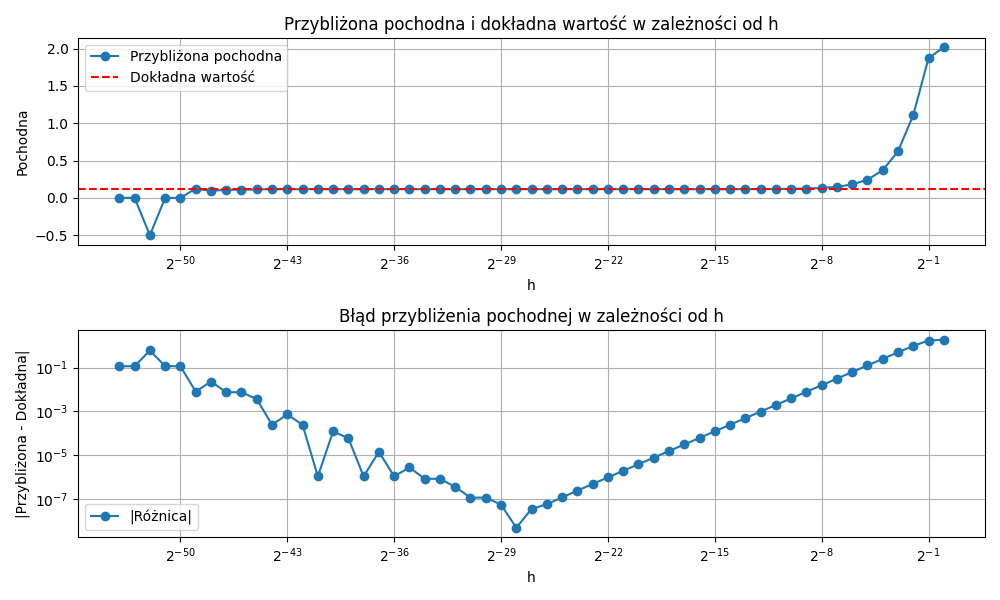
\includegraphics[width=\textwidth]{/home/wojteq18/sem5/ON/Lab/Lista1/wykres.png}

Dokładną wartość pochodnej możemy uzyskać obliczając: $\frac{d}{dx} sin(x) + cos (3x) = cos(x) - 3sin(3x)$

Analizując otrzymane wyniki, widzimy, że początkowo wraz ze zmniejszeniem wartości h, błąd przybliżenia pochodnej maleje. Jednak od około $ h = 2^{-27}$ błąd zaczyna 
rosnąć, wraz ze zmniejszaniem wartości h. Jest to spowodowane błędami zaokrągleń. Gdy h jest bardzo małe, różnica $f(x+h) - f(x)$ staje się bardzo mała i jest
reprezentowana z ograniczoną precyzją w arytmetyce zmiennoprzecinkowej. 

\begin{table}[h!]
    \centering
    \begin{tabular}{|c|c|c|}
        \hline
        $h$ & $\tilde{f}'(x_0)$ & Błąd bezwzględny \\
        \hline
        $2^{0}$ & $2.017989$ & $1.901047$ \\
        \hline
        $2^{-1}$ & $1.870441$ & $1.753499$ \\
        \hline
        $2^{-2}$ & $1.107787$ & $0.990845$ \\
        \hline
        $2^{-3}$ & $0.623241$ & $0.506299$ \\
        \hline
        $2^{-4}$ & $0.370400$ & $0.253458$ \\
        \hline
        $2^{-5}$ & $0.243443$ & $0.126501$ \\
        \hline
        $2^{-6}$ & $0.180098$ & $0.0631553$ \\
        \hline
        $2^{-7}$ & $0.148491$ & $0.0315491$ \\
        \hline
        $2^{-8}$ & $0.132709$ & $0.0157668$ \\
        \hline
        $2^{-9}$ & $0.124824$ & $0.00788141$ \\
        \hline
        $2^{-10}$ & $0.120882$ & $0.00394020$ \\
        \hline
        $2^{-11}$ & $0.118912$ & $0.00196997$ \\
        \hline
        $2^{-12}$ & $0.117927$ & $0.000984952$ \\
        \hline
        $2^{-13}$ & $0.117435$ & $0.000492468$ \\
        \hline
        \dots & \dots & \dots \\
        \hline
        $2^{-50}$ & $0.0$ & $0.116942$ \\
        \hline
        $2^{-51}$ & $0.0$ & $0.116942$ \\
        \hline
        $2^{-52}$ & $-0.5$ & $0.616942$ \\
        \hline
        $2^{-53}$ & $0.0$ & $0.116942$ \\
        \hline
        $2^{-54}$ & $0.0$ & $0.116942$ \\
        \hline
    \end{tabular}
    \caption{Przybliżone wartości pochodnej i błędy bezwzględne dla różnych $h$ (nowe dane)}
    \label{tab:pochodna_new}
\end{table}


\end{document}